%%%%%%%%%%%%%%%%%%%%%%%%%%%%%%%%%%%%%%%%%
% Wenneker Article
% LaTeX Template
% Version 2.0 (28/2/17)
%
% This template was downloaded from:
% http://www.LaTeXTemplates.com
%
% Authors:
% Vel (vel@LaTeXTemplates.com)
% Frits Wenneker
%
% License:
% CC BY-NC-SA 3.0 (http://creativecommons.org/licenses/by-nc-sa/3.0/)
%
%%%%%%%%%%%%%%%%%%%%%%%%%%%%%%%%%%%%%%%%%

%----------------------------------------------------------------------------------------
%	PACKAGES AND OTHER DOCUMENT CONFIGURATIONS
%----------------------------------------------------------------------------------------

\documentclass[10pt, a4paper, twocolumn]{article} % 10pt font size (11 and 12 also possible), A4 paper (letterpaper for US letter) and two column layout (remove for one column)

\usepackage[english]{babel} % English language hyphenation
\usepackage{microtype} % Better typography
\usepackage{amsmath,amsfonts,amsthm} % Math packages for equations
\usepackage[svgnames]{xcolor} % Enabling colors by their 'svgnames'
\usepackage[hang, small, labelfont=bf, up, textfont=it]{caption} % Custom captions under/above tables and figures
\usepackage{booktabs} % Horizontal rules in tables
\usepackage{lastpage} % Used to determine the number of pages in the document (for "Page X of Total")
\usepackage{graphicx} % Required for adding images
\usepackage{amssymb}
\usepackage[table]{xcolor}
\usepackage{enumitem} % Required for customising lists
\setlist{noitemsep} % Remove spacing between bullet/numbered list elements
\usepackage{sectsty} % Enables custom section titles
\allsectionsfont{\usefont{OT1}{phv}{b}{n}} % Change the font of all section commands (Helvetica)
\usepackage{hyperref}
%----------------------------------------------------------------------------------------
%	MARGINS AND SPACING
%----------------------------------------------------------------------------------------
\usepackage{geometry} % Required for adjusting page dimensions
\geometry{
	top=0.65cm, % Top margin
	bottom=1.5cm, % Bottom margin
	left=1.5cm, % Left margin
	right=1.5cm, % Right margin
	includehead, % Include space for a header
	includefoot, % Include space for a footer
	%showframe, % Uncomment to show how the type block is set on the page
}
\setlength{\columnsep}{6mm} % Column separation width


%----------------------------------------------------------------------------------------
%	FONTS
%----------------------------------------------------------------------------------------

\usepackage[T1]{fontenc} % Output font encoding for international characters
\usepackage[utf8]{inputenc} % Required for inputting international characters

\usepackage{XCharter} % Use the XCharter font



%\input{structure.tex} % Specifies the document structure and loads requires packages

%----------------------------------------------------------------------------------------
%	ARTICLE INFORMATION
%----------------------------------------------------------------------------------------

\title{Robhoot 1.0\\ The Deep Knowledge Network} % The article title
  \author{XX{\textsuperscript{1,2,3} and XY\textsuperscript{2,3}} % Authors
  \newline\newline % Space before institutions
  \\
	\textsuperscript{1}\institution{}\\ % Institution 1
	\textsuperscript{2}\institution{}\\ % Institution 2
	%\textsuperscript{3}\institution{\texttt{LaTeXTemplates.com}}
      %} % Institution 3


% Example of a one line author/institution relationship
%\author{\newauthor{John Marston} \newinstitution{Universidad Nacional Autónoma de México, Mexico City, Mexico}}

\date{\today} % Add a date here if you would like one to appear underneath the title block, use \today for the current date, leave empty for no date
%---------------------------------------------------------------------------------------

\begin{document}

\maketitle % Print the title
\thispagestyle{firstpage} % Apply the page style for the first page (no headers and footers)

%----------------------------------------------------------------------------------------
%	ABSTRACT
%----------------------------------------------------------------------------------------
\lettrineabstract{\section{{\bf Summary}} The Robhoot project aims to
  connect research and the public in a decentralized network to help
  taking informed decisions when solving complex social, environmental
  and technological problems. Current technologies for scientific
  inquiry and decision-making are highly fragmented and thus only
  increase robustness, reproducibility, open-access and the
  interactions with the public marginally. The goal of Robhoot is to
  propose a hybrid-technology to lay out the foundation for a
  open-science research ecosystem aiming to strengthen the robustness
  and reproducibility of science and the interactions with the
  public. Robhoot is not set out to deliver a finished deep knowledge
  network in the science ecosystem, but to provide a science-enabled
  technology in establishing a prototype proof-of-principle to connect
  decentralized and neutral-knowledge generation with
  knowledge-inspired societies.}
%----------------------------------------------------------------------------------------
%	ARTICLE CONTENTS
%----------------------------------------------------------------------------------------
\section{The Science Ecosystem}
The process of science requires multiple steps of information transfer
among trusted/untrusted peers to build solid evidence-based knowledge
in social, economical, natural and technological ecosystems. Solid
evidence-based knowledge should be immutable and have a secure
peer-to-peer architecture storing the open-source knowledge graphs
derived from the research output. These steps are key to have fully
reproducible open-access reports when taking informed decisions in
complex societal, environmental and technological problems. However,
public funded science is highly centralized (Günther, 2018; Inhaber,
1977)⁠⁠, prone to errors ((Fang & Casadevall, 2011)⁠), difficult to
reproduce (Hardwicke. et al., 2019)), and contains many biases
(Ioannidis, 2005). These elements make the connection between the
scientific process and open-access reporting for decision-making
highly improbable. Despite many projects are aiming at making the
science ecosystem less centralized and biased while increasing
openness and reproducibility (refs) a science-enabled technological
paradigm connecting open-science to knowledge-inspired societies is
not currently in place.

Many studies in decentralized systems are producing an immense gain in
detailed knowledge about scalability, security and decentralization
trade-offs (refs; TON network; Fabric ledger OS network). Automation
and AI technologies is the other angle from which many advances are
rapidly occurring (refs). Yet, while the existing technological
paradigm is rapidly shifting towards science-based decentralization
and automation technologies, end-to-end open-source research
accounting for decentralized, neutral and automated knowledge-inspired
technologies are missing. Rapid advances of automated research
platforms facilitating data integration accounting for sections of the
research cycle are currently under development\footnote{This is by no
  means an exhaustive list but it gives an indication of the many
  projects currently in place:
  \href{https://www.nterminal.com}{NakamotoT},\href{https://cloud.google.com/bigquery/}{BigQuery},\href{https://www.automaticstatistician.com/index/}{Automated
    statistician},\href{http://www.modulos.ai/}{Modulos},\href{https://ai.google/}{Google
    AI},\href{https://iris.ai}{Iris},\href{https://github.com/DS3Lab/easeml}{easeml}}
but open-source decentralized automated platforms accounting for the
research cycle are still at a very incipient stage of development. While conceptual frameworks conceptualizing the required layers in
many research fields are well established (Figure 1a), there is
currently a lack of tools automating the knowledge graphs (Figure 1b)
into deep process-based learning networks exploring its
robustness (Figure 1c) and decentralization power (Figure 1d).

\begin{table}
 %\rowcolor{pink}
\begin{tabular}{ p{3cm} | p{2cm} | p{2cm}}
  \hline \hline
  \textbf{Features} & \textbf{Science Ecosystem} &\textbf{Robhoot 1.0}\\  \hline
  Decentralization & No & Yes \\ \hline
  Open-access & Mostly No & Yes \\ \hline
  Immutability & No & Yes \\ \hline
  Robustness & Mostly No & Yes \\ \hline
  Reproducibility & Mostly No & Yes \\ \hline        
  Owner-Controlled assets & No & Yes \\ \hline       
  \bottomrule

\end{tabular}
\caption{Robhoot 1.0 aims to be designed to resolve desirable
  properties of science: Robustness, Reproducibility,
  Decentralization, Open and Direct access to reporting by peers and
  not-peers}
\end{table}
% ------------------------------------------------
  \section{Robhoot Design Goals}
  Robhoot aims to build an automated knowledge network technology to
  connect knowledge-graphs to knowledge-inspired societies (Figure
  1). Our final aim is to provide real-time open-access neutral
  data-rule-knowledge to gain informed decisions when solving complex
  social, environmental and technological problems.
  \includegraphics[width=0.45\textwidth]{Figure1.pdf}
  
  {\small {\bf Figure 1: Deep knowledge-based ledger network
      technology}. a) End-to-end research cycle from data integration
    (top) to reporting (bottom). b) The knowledge graph (KG) tracking
    one research path of a (i.e., Renku open-source code). c) Deep
    knowledge-based network automatically exploring a population of
    KGs to gain process-based understanding of the data. d) The ledger
    accounts for all the KGs in a distributed network of mutually
    trusting/untrusting peers with every peer maintaining the
    population of the KGs (i.e., decentralized P2P git network like
    Gitchain.)}  The overall objectives for the project are the
  following:
  \subsection{Deep learning networks}
  \begin{itemize}
  \item Deploy an automated knowledge-based network technology
    accounting for end-to-end research in a lineage client-tracker to
    produce a population of Knowledge Graphs (KGs) (Figures 1a-b).
  \item Intralayer automation of data integration, inference, and
    validation (Figure 1a: top four layers).
  \item Intralayer automation of visualization and reporting
    generation (Figure 1a: bottom two layers).
  \item Deep inter-layer automation exploring novel neural biological
    networks algorithms with lineage client-tracker paths in the
    multilayer network (Figures 1a-c.)
  \end{itemize}
  \subsection{Distributed ledger network}
  \begin{itemize}
  \item Deploy an end-to-end permissioned-permissionless distributed
    ledger technology to guarantee decentralization, open-access and
    security of the KGs populations in the science ecosystem (Figures
    1c and 1d.)
  \item Distributed ledger implementation accounting for consensus
    algorithms and smart contracts among trusted-untrusted
    peer-to-peer interactions.
  \item Exploring consensus algorithms to minimize
    scalability-security-decentralization trade-offs when storing the
    KGs in the knowledge network.
  \end{itemize}
  \subsection{DeepKlen 1.0}  
  \begin{itemize}
  \item Testnet for the interaction between consensus protocols and
    the scalability-security-decentralization trade-offs when
    committing the KGs to the distributed ledger.
  \item Mainnet to cryptographically link each population of KGs to
    previous KGs-ledger to create an historical KGs-ledger chain that
    goes back to the genesis ledger. The mainnet aims to connect
    database real-time open-access citizen data science to
    knowledge-inspired societies.
  \end{itemize}
 \subsection{Robhoot 1.0}
 \begin{itemize}
 \item Robhoot Open Network in Biodiversity Research to connect
   citizen open science to real-time open-access data-rule-knowledge
   to gain informed decisions when solving local and global
   environmental problems.
 \item Citizen open science for biodiversity datasets integration.
\end{itemize}
%------------------------------------------------
\section{The multilayer nature of Robhoot}

\subsection{Data integration}
\subsection{Complexity reduction}
\subsection{Inference}
\subsection{Validation}
\subsection{Visualization}
\subsection{Reporting}

\section{Robhoot in Digital Ecosystems}

\subsection{Computing Power}
\subsection{Decentralization}
\subsection{Neural Networks}

\section{How to contribute to Robhoot}

\section{The Robhoot roadmap}

\includegraphics[width=1\textwidth]{GanttChart.pdf}

{\small {\bf Figure 2: The Robhoot roadmap}}




\section{Conclusion}


%----------------------------------------------------------------------------------------
%	BIBLIOGRAPHY
%----------------------------------------------------------------------------------------

\printbibliography[title={Bibliography}] % Print the bibliography, section title in curly brackets

%----------------------------------------------------------------------------------------

\end{document}

\hspace{-0.2 in}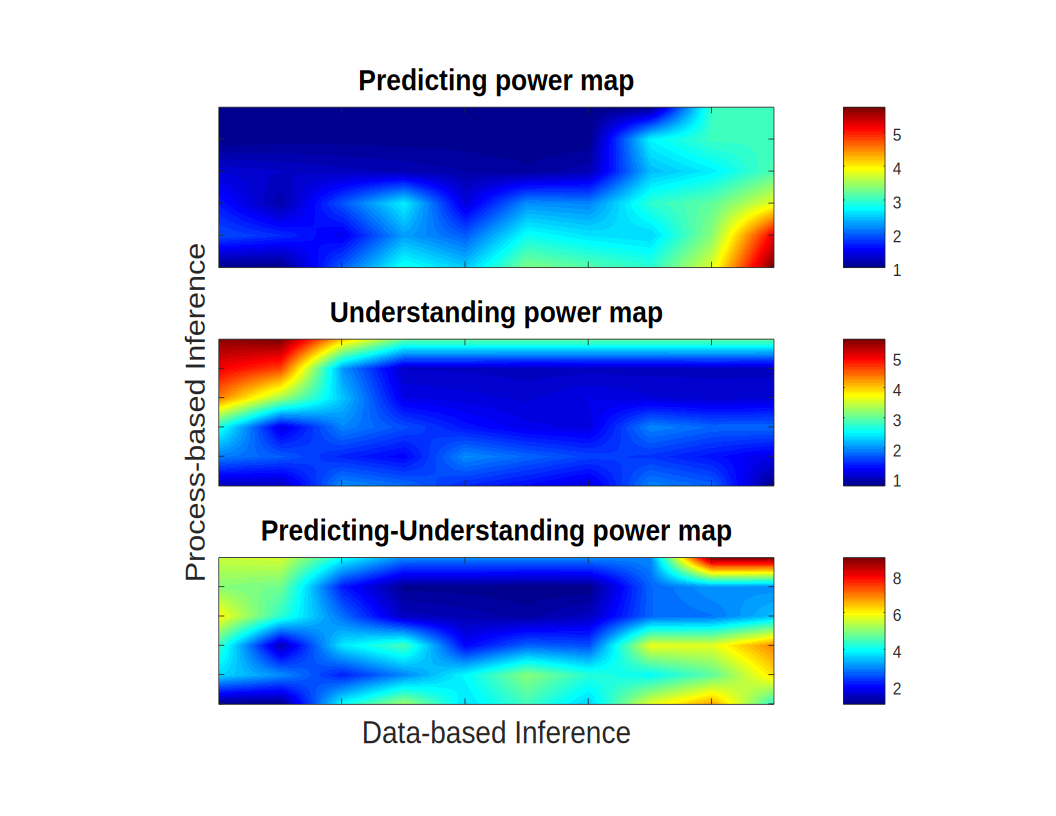
\includegraphics[width=0.52\textwidth]{Figure3.pdf}
{\small {\bf Figure 1: Prediction power (top), understanding (middle),
    and prediction-understanding power maps (bottom)}. x-axis
  represents data-based inference (i.e., gradient of AI methods from
  low (left) to high (right) predictive power). y-axis represents
  process-based inference (i.e., gradient of process-based methods
  from low (bottom left) to high (top left) understanding power). The
  gradient of predicting power map (top) shows a hot spot red area in
  the bottom right highlighting the region where AI methods best
  predict the empirical data. The gradient of understanding power map
  (middle) shows a red hot spot in the top left highlighting the
  region where the best mechanistic understanding occur. The
  predicting-understanding power map (bottom) shows the sum of the two
  previous maps highlighting a red hot spot where the best synthesis
  research joining predicting and understanding power of the empirical
  data might occur. The first research goal of this proposal aims to
  build an automated research platform to maximize the predicting and
  understanding power highlighted in the red hot spot of the
  predicting-understanding power map (bottom).}
